
\subsection{LHC chamber with sawtooth structure}
The transverse geometry of the LHC chamber is pictured in Fig.~\ref{fig:beam_screen_structure}.
Of great importance is the sawtooth structure that ensures an almost normal impact of most photons on the surface, greatly reducing the reflectivity.
Therefore, most photoelectrons are created at the outer part of the beam screens, where they do not significantly contribute to the electron cloud buildup.


\begin{figure}[tbh]
    \centering
    \begin{minipage}[c]{0.47\textwidth}
        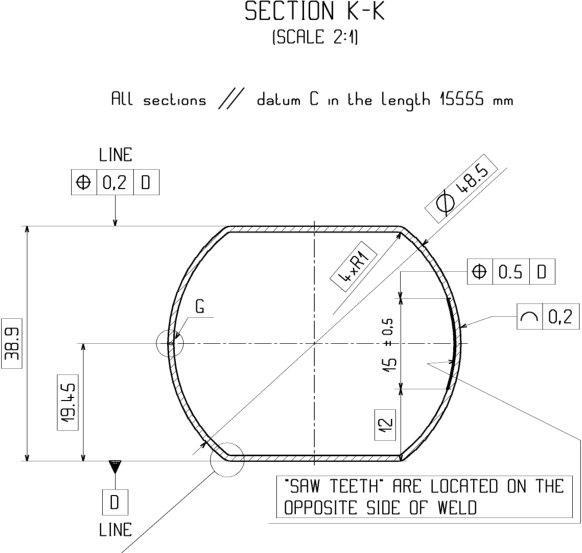
\includegraphics[width=\textwidth]{../ss/beam_screen_drawing.png}
    \end{minipage}
    \hspace{0.5cm}
    \begin{minipage}[c]{0.47\textwidth}
        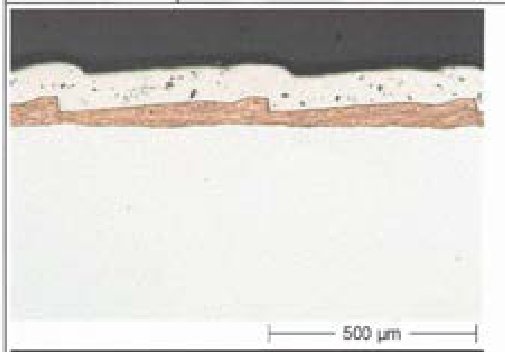
\includegraphics[width=\textwidth]{../ss/sawtooth_fine.png}
    \end{minipage}
\caption{
		Left: the technical drawing of the LHC beam screen~\cite{beam_screen_drawing}. Right: a closeup of the sawtooth structure. The vertical edges are about 35~$\mu$m long~\cite{zimmermann}.
		}
\label{fig:beam_screen_structure}
\end{figure}


\subsection{SynRad3D simulations}
The azimuthal distributions of absorbed photons in the LHC chamber have been simulated with the code SynRad3D~\cite{guillermo}.
The photons origin from a beam with 7~TeV energy, and only photons with more than 4~eV energy are considered.
The results are shown in Fig.~\ref{fig:guillermo}.
With access to the raw data, it could be converted to the PyECLOUD input parameter \textbf{inv\_CDF\_refl\_photoem\_file}.

\begin{figure}[tbh]
    \centering
    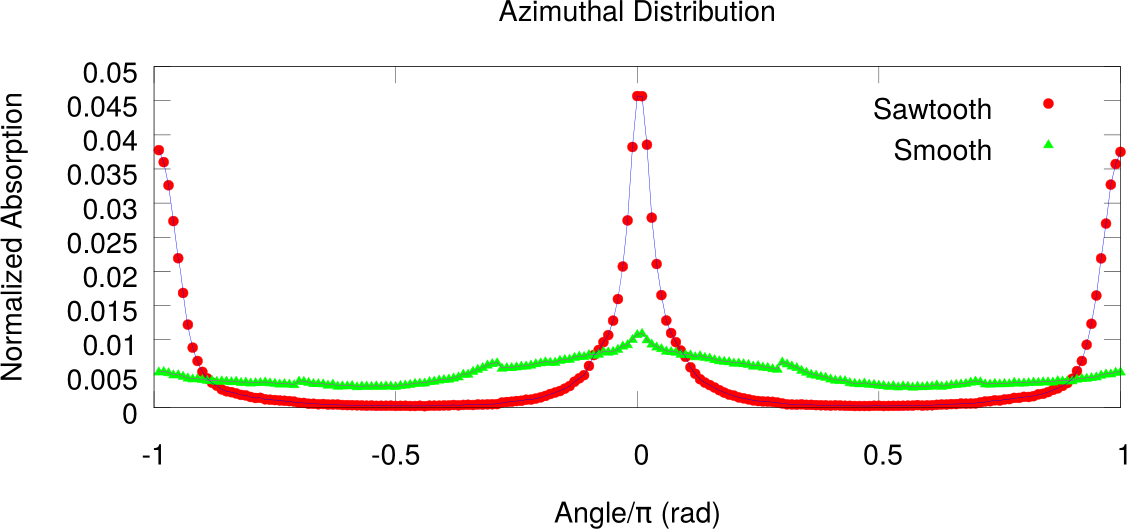
\includegraphics[width=0.8\textwidth]{../ss/photon_distribution_guillermo.png}
	\caption{The photon distribution as it was simulated for the LHC chamber geometry with and without sawtooth~\cite{guillermo}.
	An angle of 0 corresponds to the impact point of the synchrotron radiation.}
    \label{fig:guillermo}
\end{figure}


\subsection{Other simulations}

